\documentclass{ntuabeamer}

\usepackage[utf8]{inputenc}
\usepackage{amsmath}
\usepackage{amssymb}
\usepackage{booktabs}
\usepackage{graphicx}
\usepackage{tikz}
\usetikzlibrary{arrows.meta,positioning}

\title{Supervised Learning Fundamentals}
\author{}
\date{}

\graphicspath{{assets/}{assets/generated/}}

\definecolor{courseblue}{HTML}{3F7CAC}
\definecolor{courseorange}{HTML}{D97706}
\definecolor{coursegreen}{HTML}{27864A}
\definecolor{coursegray}{HTML}{667085}
\definecolor{courselightblue}{HTML}{DCE9F5}
\definecolor{courselightorange}{HTML}{F9E4C8}

\begin{document}

\begin{frame}[plain]
  \makepresentationtitle
\end{frame}

\begin{frame}{A Supervised-Learning Problem}
  \[
    \mathcal{D}=\{(\mathbf{x}_i,y_i)\}_{i=1}^{n},
    \qquad \mathbf{x}_i\in\mathbb{R}^{d}
  \]
  \begin{itemize}
    \item \textbf{Input} $\mathbf{x}_i$: measured features.
    \item \textbf{Target} $y_i$: desired answer.
    \item \textbf{Model} $f_{\boldsymbol{\theta}}$: parametrized prediction rule.
    \item \textbf{Prediction} $\hat y_i=f_{\boldsymbol{\theta}}(\mathbf{x}_i)$.
  \end{itemize}
\end{frame}

\begin{frame}{Learning Connects Data to an Objective}
  \centering
  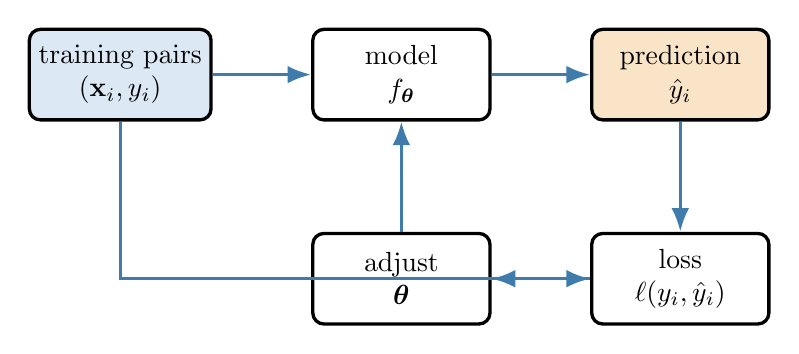
\begin{tikzpicture}[
    node distance=1.25cm,
    box/.style={draw, rounded corners, minimum width=2.25cm, minimum height=1.15cm, align=center, very thick},
    flow/.style={-{Latex[length=3mm]}, very thick, courseblue}
  ]
    \node[box, fill=courselightblue] (data) {training pairs\\$(\mathbf{x}_i,y_i)$};
    \node[box, fill=white, right=of data] (model) {model\\$f_{\boldsymbol{\theta}}$};
    \node[box, fill=courselightorange, right=of model] (prediction) {prediction\\$\hat y_i$};
    \node[box, fill=white, below=1.4cm of prediction] (loss) {loss\\$\ell(y_i,\hat y_i)$};
    \node[box, fill=white, below=1.4cm of model] (adjust) {adjust\\$\boldsymbol{\theta}$};
    \draw[flow] (data) -- (model);
    \draw[flow] (model) -- (prediction);
    \draw[flow] (prediction) -- (loss);
    \draw[flow] (data.south) |- (loss.west);
    \draw[flow] (loss) -- (adjust);
    \draw[flow] (adjust) -- (model);
  \end{tikzpicture}
  \vspace{0.35cm}
  \[
    \mathcal{L}(\boldsymbol{\theta})
    =\frac{1}{n}\sum_{i=1}^{n}
    \ell\!\left(y_i,f_{\boldsymbol{\theta}}(\mathbf{x}_i)\right)
  \]
\end{frame}

\begin{frame}{Regression Predicts a Numerical Value}
  \[
    y_i\in\mathbb{R},
    \qquad
    \hat y_i=\mathbf{w}^{\top}\mathbf{x}_i+b
  \]
  \begin{itemize}
    \item The weights $\mathbf{w}\in\mathbb{R}^{d}$ set feature contributions.
    \item The bias $b\in\mathbb{R}$ shifts every prediction.
    \item Examples include price, temperature, displacement, and stress.
  \end{itemize}
\end{frame}

\begin{frame}{Linear Regression Fits a Trend}
  \centering
  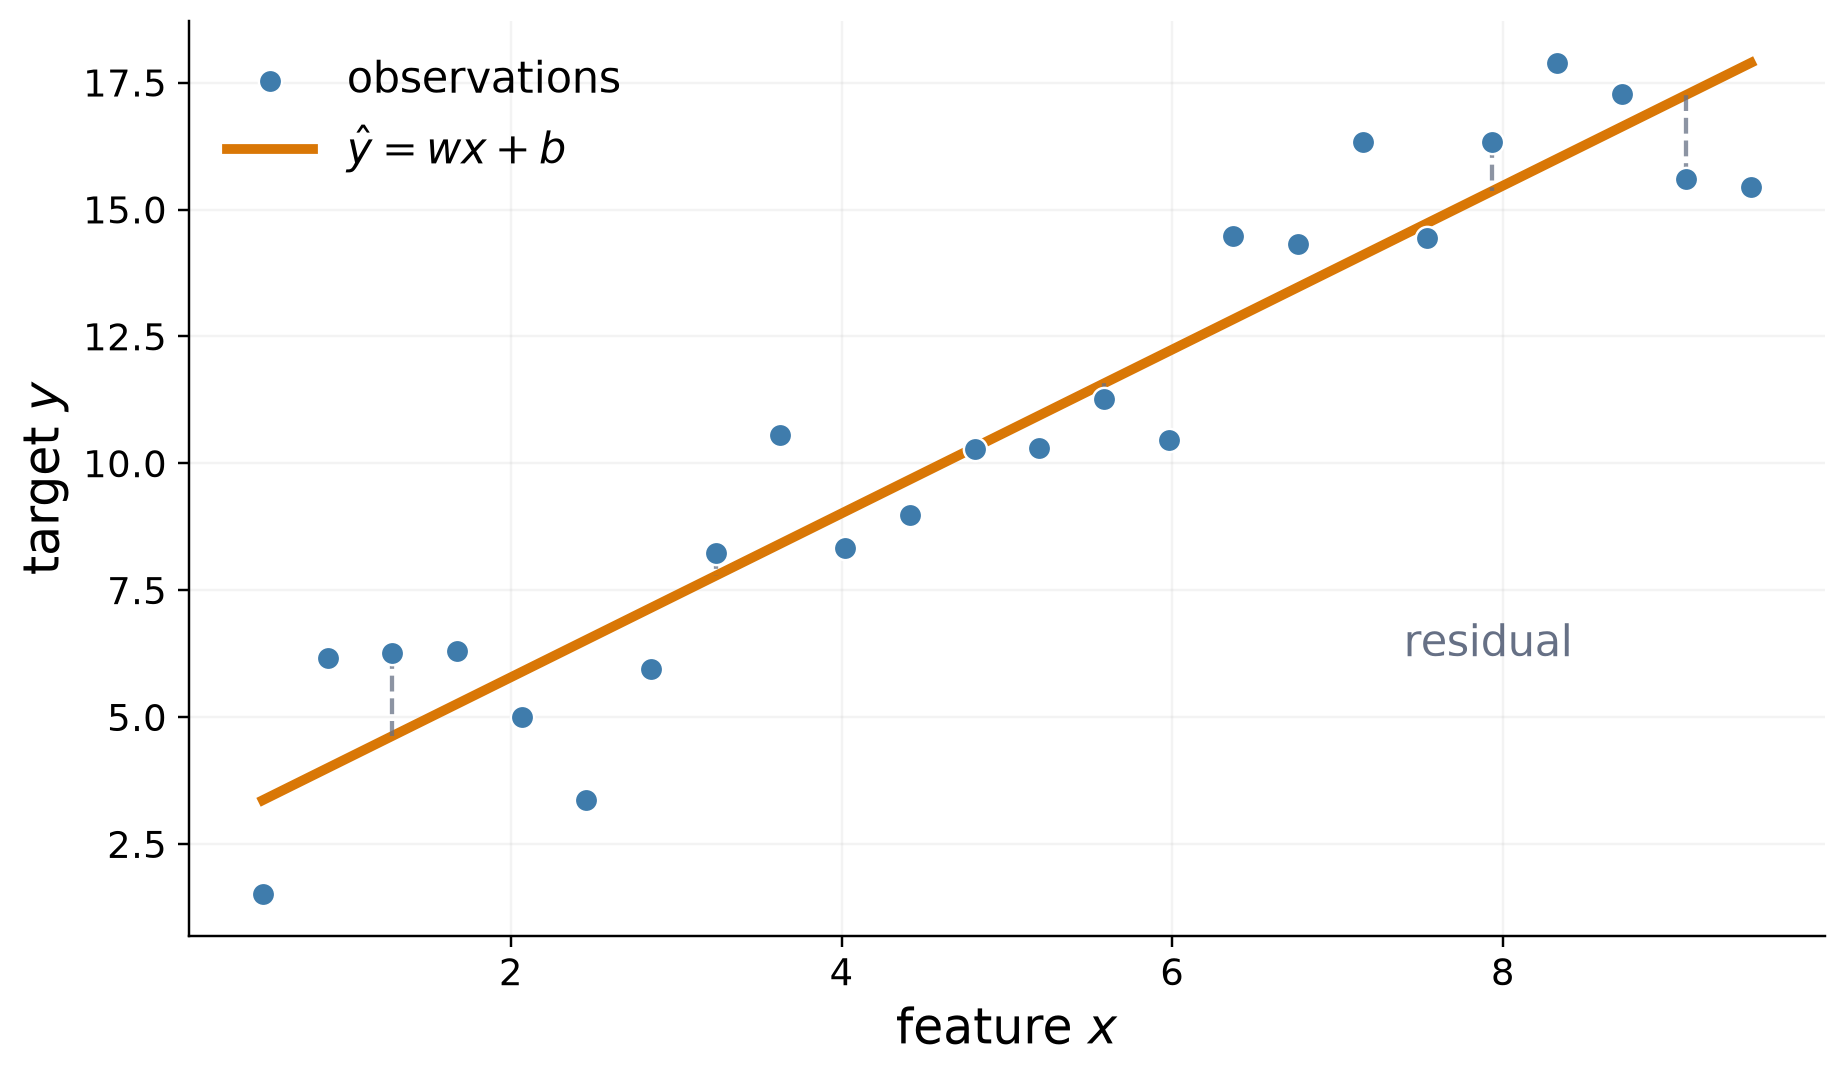
\includegraphics[width=0.94\linewidth,height=0.76\textheight,keepaspectratio]{linear-regression.png}
\end{frame}

\begin{frame}{Mean-Squared Error Penalizes Residuals}
  \[
    r_i=y_i-\hat y_i,
    \qquad
    \mathcal{L}_{\mathrm{MSE}}(\mathbf{w},b)
    =\frac{1}{n}\sum_{i=1}^{n}r_i^2
  \]
  \begin{itemize}
    \item A residual is the vertical prediction error.
    \item Squaring makes large errors more influential.
    \item Minimizing MSE estimates the linear parameters.
  \end{itemize}
\end{frame}

\begin{frame}{Binary Classification Predicts a Probability}
  \[
    y_i\in\{0,1\},
    \qquad
    \hat p_i=P(y_i=1\mid\mathbf{x}_i)
  \]
  \[
    \hat p_i=\sigma(z_i),
    \qquad
    z_i=\mathbf{w}^{\top}\mathbf{x}_i+b,
    \qquad
    \sigma(z)=\frac{1}{1+e^{-z}}
  \]
  \begin{itemize}
    \item The threshold $\hat p_i\geq 0.5$ corresponds to $z_i\geq 0$.
    \item The threshold may change when error costs are unequal.
  \end{itemize}
\end{frame}

\begin{frame}{Logistic Regression Learns a Decision Boundary}
  \centering
  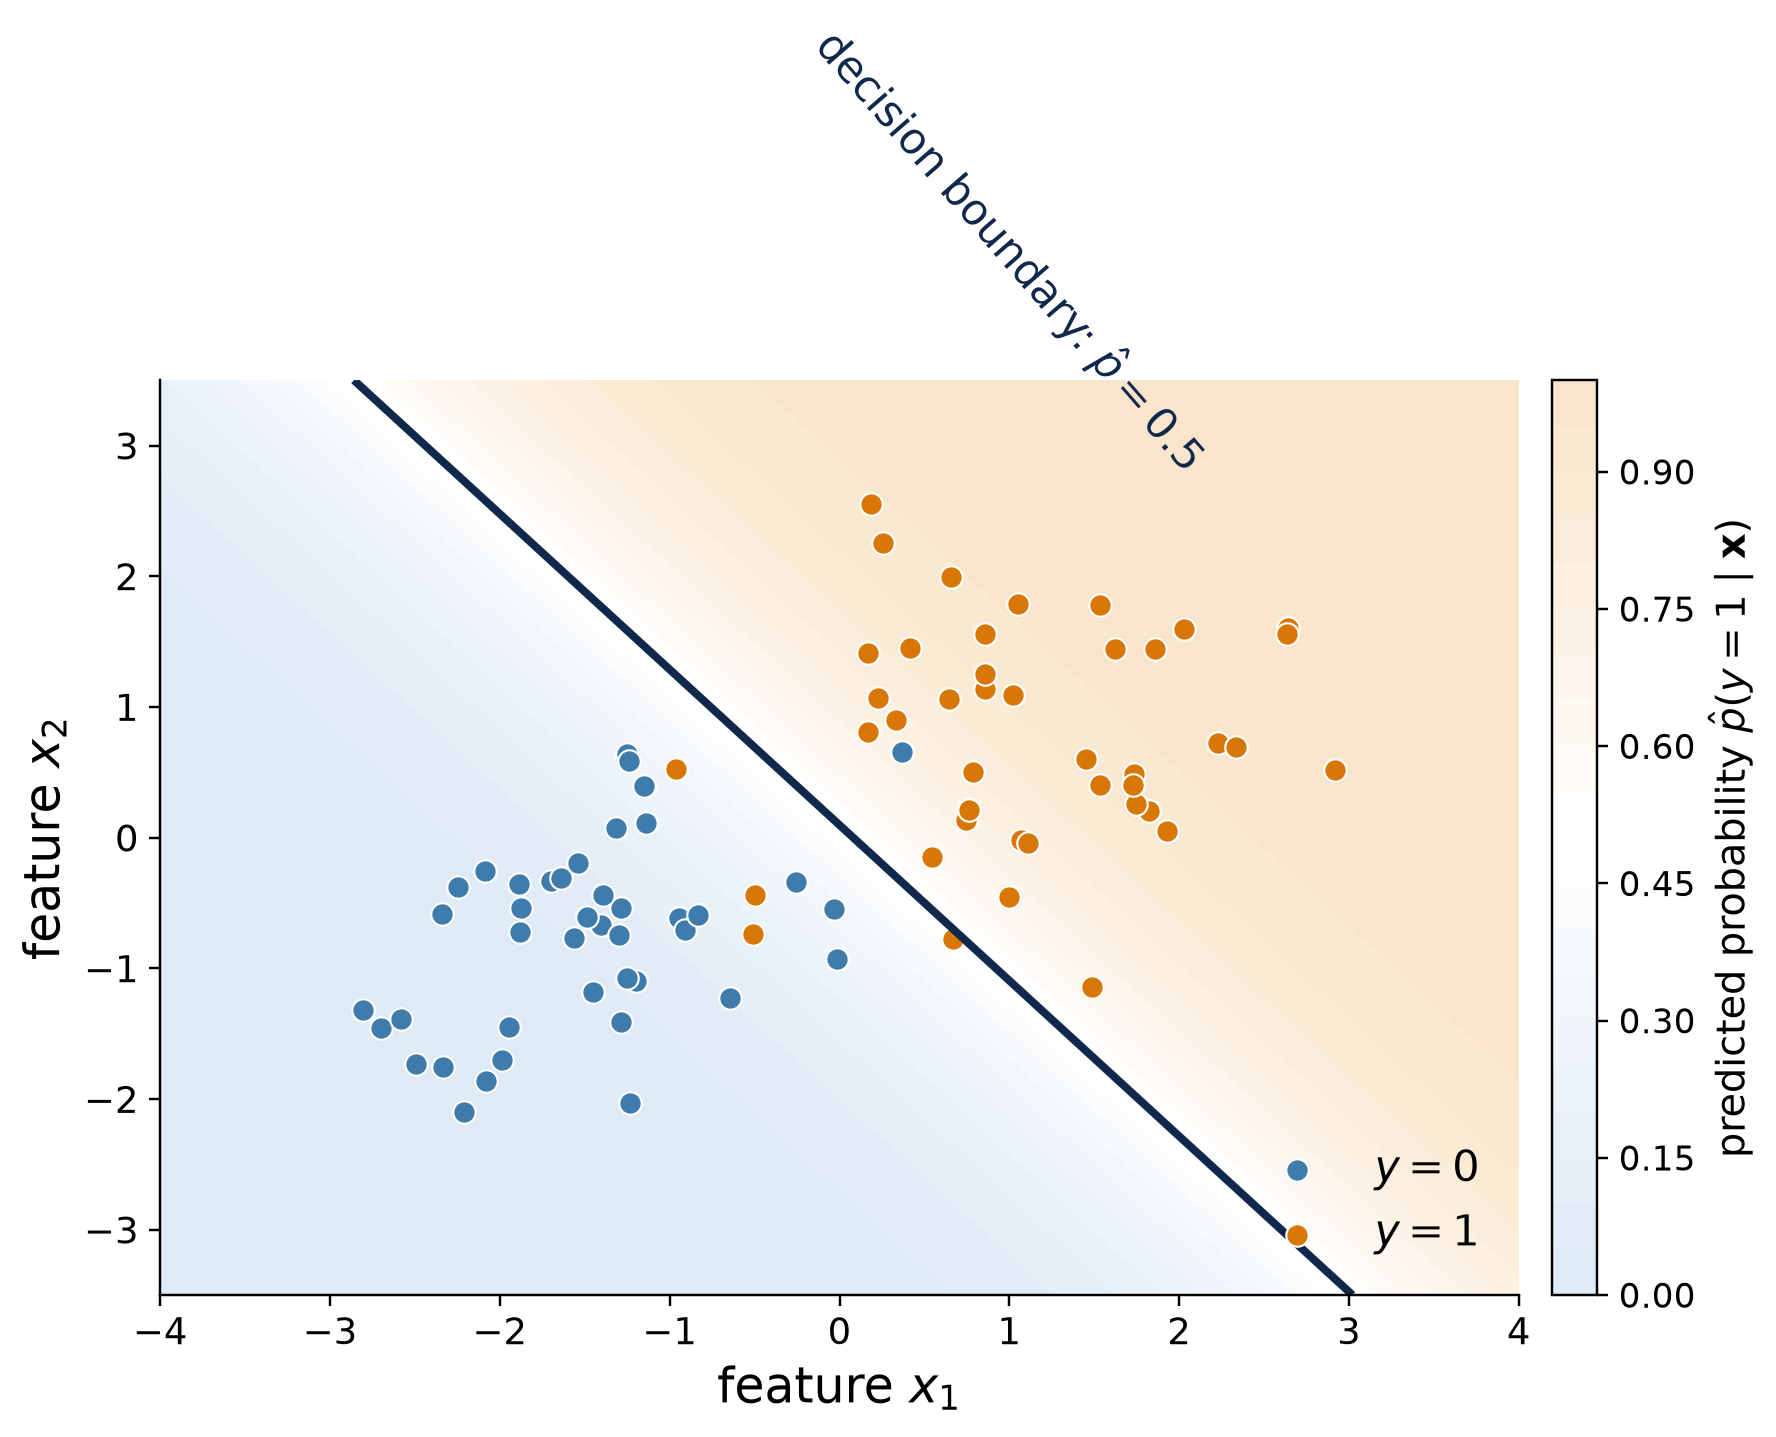
\includegraphics[width=0.95\linewidth,height=0.78\textheight,keepaspectratio]{logistic-regression.png}
\end{frame}

\begin{frame}{Cross-Entropy Scores Probabilities}
  \[
    \ell_{\mathrm{BCE}}(y_i,\hat p_i)
    =-y_i\log\hat p_i-(1-y_i)\log(1-\hat p_i)
  \]
  \[
    \mathcal{L}_{\mathrm{BCE}}(\mathbf{w},b)
    =\frac{1}{n}\sum_{i=1}^{n}
    \ell_{\mathrm{BCE}}(y_i,\hat p_i)
  \]
  \begin{itemize}
    \item Confident wrong predictions receive a large penalty.
    \item Accurate probabilities receive a small penalty.
  \end{itemize}
\end{frame}

\begin{frame}{Split Before Fitting Anything}
  \centering
  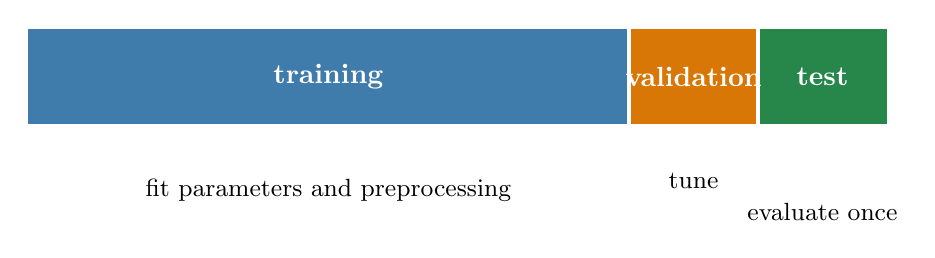
\begin{tikzpicture}[x=0.09\textwidth,y=1cm]
    \fill[courseblue] (0,0) rectangle (7,1.2);
    \fill[courseorange] (7,0) rectangle (8.5,1.2);
    \fill[coursegreen] (8.5,0) rectangle (10,1.2);
    \draw[white,very thick] (7,0) -- (7,1.2);
    \draw[white,very thick] (8.5,0) -- (8.5,1.2);
    \node[white,font=\bfseries] at (3.5,0.6) {training};
    \node[white,font=\bfseries] at (7.75,0.6) {validation};
    \node[white,font=\bfseries] at (9.25,0.6) {test};
    \node[align=center,font=\small] at (3.5,-0.85) {fit parameters and preprocessing};
    \node[align=center,font=\small] at (7.75,-0.72) {tune};
    \node[align=center,font=\small] at (9.25,-1.12) {evaluate once};
  \end{tikzpicture}
\end{frame}

\begin{frame}{Leakage Makes Evaluation Optimistic}
  \centering
  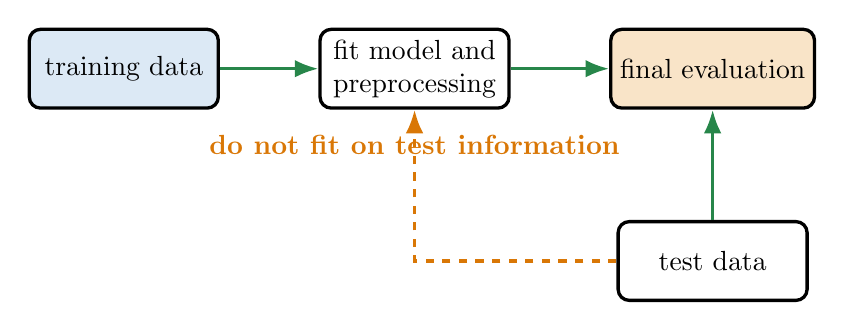
\begin{tikzpicture}[
    node distance=1.25cm,
    box/.style={draw, rounded corners, minimum width=2.4cm, minimum height=1.0cm, align=center, very thick},
    good/.style={-{Latex[length=3mm]}, very thick, coursegreen},
    bad/.style={-{Latex[length=3mm]}, very thick, courseorange, dashed}
  ]
    \node[box,fill=courselightblue] (train) {training data};
    \node[box,fill=white,right=of train] (fit) {fit model and\\preprocessing};
    \node[box,fill=courselightorange,right=of fit] (evaluate) {final evaluation};
    \node[box,fill=white,below=1.4cm of evaluate] (test) {test data};
    \draw[good] (train) -- (fit);
    \draw[good] (fit) -- (evaluate);
    \draw[good] (test) -- (evaluate);
    \draw[bad] (test.west) -| (fit.south);
    \node[courseorange,font=\bfseries,below=0.2cm of fit] {do not fit on test information};
  \end{tikzpicture}
\end{frame}

\begin{frame}{Loss Trains; Metrics Communicate}
  \centering
  \begin{tabular}{lll}
    \toprule
    \textbf{Task} & \textbf{Training loss} & \textbf{Evaluation metrics} \\
    \midrule
    Regression & MSE & MAE, RMSE, $R^2$ \\
    Binary classification & Cross-entropy & Accuracy, precision, recall \\
    \bottomrule
  \end{tabular}
  \vspace{0.6cm}
  \begin{itemize}
    \item A loss must support parameter optimization.
    \item A metric should answer the application question.
    \item Report more than one metric when error types differ.
  \end{itemize}
\end{frame}

\begin{frame}{Normalize With Training Statistics Only}
  \[
    \mu_j^{\mathrm{train}}
    =\frac{1}{n_{\mathrm{train}}}\sum_{i\in\mathrm{train}}x_{ij},
    \qquad
    \sigma_j^{\mathrm{train}}
    =\sqrt{\frac{1}{n_{\mathrm{train}}}
      \sum_{i\in\mathrm{train}}(x_{ij}-\mu_j^{\mathrm{train}})^2}
  \]
  \[
    \tilde x_{ij}
    =\frac{x_{ij}-\mu_j^{\mathrm{train}}}{\sigma_j^{\mathrm{train}}}
  \]
  \begin{itemize}
    \item Apply the same $\mu_j^{\mathrm{train}}$ and $\sigma_j^{\mathrm{train}}$ to every split.
    \item Never recompute preprocessing from validation or test data.
  \end{itemize}
\end{frame}

\begin{frame}{Normalization Places Features on Comparable Scales}
  \centering
  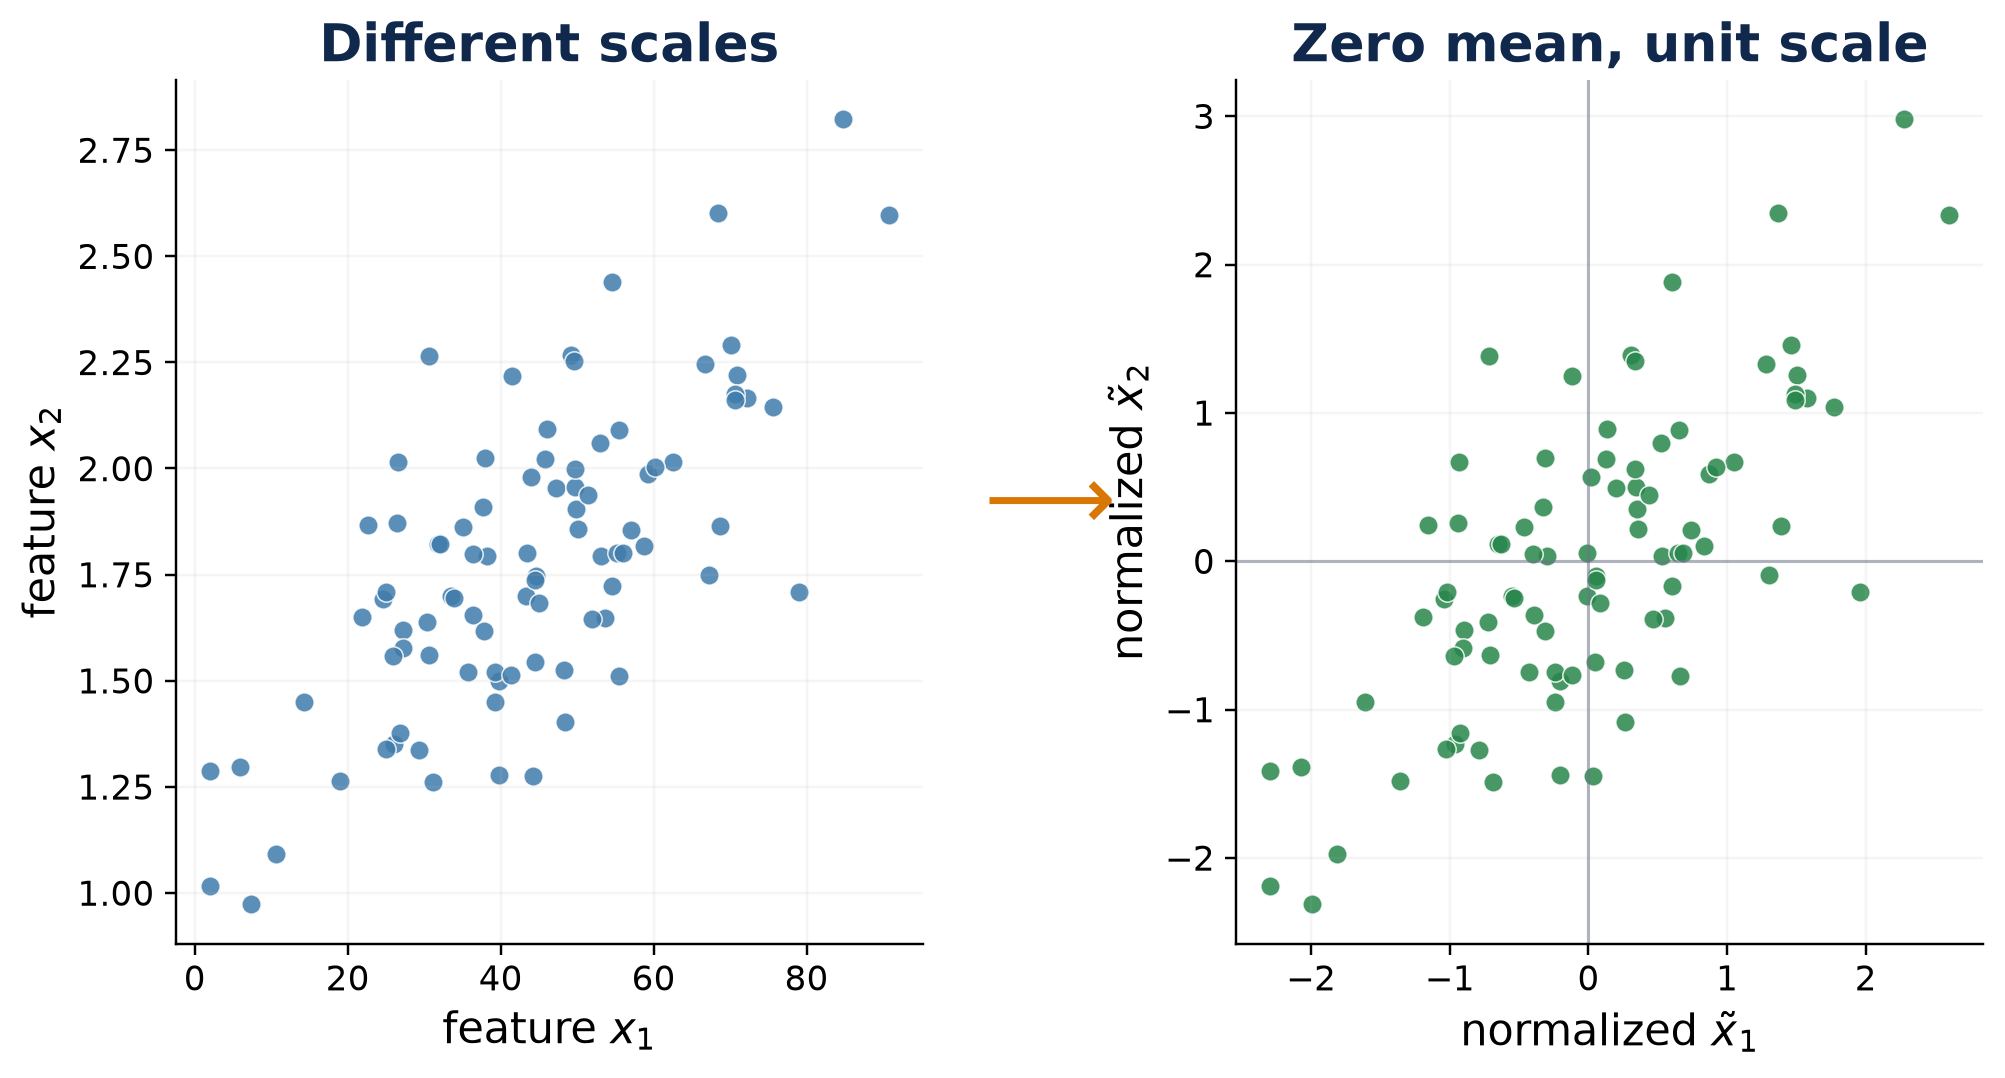
\includegraphics[width=0.97\linewidth,height=0.78\textheight,keepaspectratio]{normalization.png}
\end{frame}

\begin{frame}{One Notation Across the Course}
  \[
    \hat y_i=f_{\boldsymbol{\theta}}(\mathbf{x}_i),
    \qquad
    \mathcal{L}(\boldsymbol{\theta})
    =\frac{1}{n}\sum_{i=1}^{n}\ell(y_i,\hat y_i)
  \]
  \begin{itemize}
    \item $\mathbf{x}_i$: input features.
    \item $y_i$: observed target.
    \item $\hat y_i$: model prediction.
    \item $\boldsymbol{\theta}$: all learnable parameters.
    \item $\mathcal{L}$: empirical training objective.
  \end{itemize}
\end{frame}

\begin{frame}{Next: How Do Parameters Learn?}
  \centering
  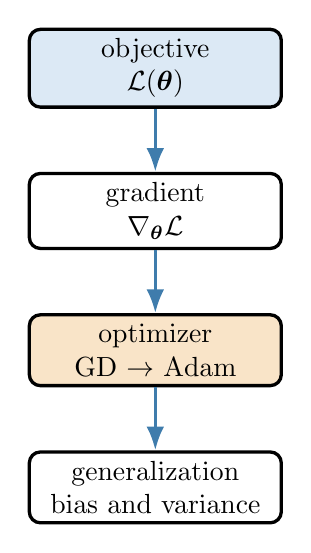
\begin{tikzpicture}[
    node distance=0.8cm,
    box/.style={draw, rounded corners, minimum width=3.2cm, minimum height=0.9cm, align=center, very thick},
    flow/.style={-{Latex[length=3mm]}, very thick, courseblue}
  ]
    \node[box,fill=courselightblue] (objective) {objective\\$\mathcal{L}(\boldsymbol{\theta})$};
    \node[box,fill=white,below=of objective] (gradient) {gradient\\$\nabla_{\boldsymbol{\theta}}\mathcal{L}$};
    \node[box,fill=courselightorange,below=of gradient] (optimizer) {optimizer\\GD $\rightarrow$ Adam};
    \node[box,fill=white,below=of optimizer] (generalization) {generalization\\bias and variance};
    \draw[flow] (objective) -- (gradient);
    \draw[flow] (gradient) -- (optimizer);
    \draw[flow] (optimizer) -- (generalization);
  \end{tikzpicture}
\end{frame}

\end{document}
